\documentclass[memoire.tex]{subfiles}

\chapter{Analyse des solutions logicielles existantes}

Maintenant que nous avons vu les différentes architecture Big Data existantes et que nous les avons décomposés, on va s'intéresser plus en détail à chaque composant de ces architecture. Pour chaque composant, nous allons présenter diverses solutions existantes permettant de remplir le rôle de ce dernier. Pour chacune de ses solutions, nous allons voir leurs avantages et inconvénients et leurs manière de fonctionner dans le but de pouvoir en dégager des critères de sélections.

\section{Message Broker}

Un Message broker~\cite{MSG_BROKER}, Agent de message en français, est un moyen de communication utilisant des messages entre deux applications (Ex: Communication entre un serveur et un client). Un message broker permet une communication asynchrone entre applications. L'utilisation de cette solution permet de pouvoir facilement filtrer les messages que l'on reçoit et de stocker temporairement les messages reçus afin d'éviter les pertes de données. Ce dernier cas, s'avère très utile dans le cas où l'application chargée de la réception des données n'est pas en fonctionnement pendant un certains temps. Il existe deux types de communications avec un message broker : 

\subsubsection*{Publisher / Subscriber}

Dans ce mécanisme, l'entité envoyant les données est nommé "Publisher" et l'entité les récupérant est nommé "Subscriber". Le publisher va envoyer des données dans des topics \footnote{Un topic est une catégorie dans laquelle les messages produit sont stockés.} afin que les Subscribers de ce topic puissent les récupérer. Un publisher peut envoyer des données dans un ou plusieurs topics, et les subscribers peuvent être abonné à un ou plusieurs topics (Voir figure 2.1). 


\begin{figure}[!h]
	\centering 
	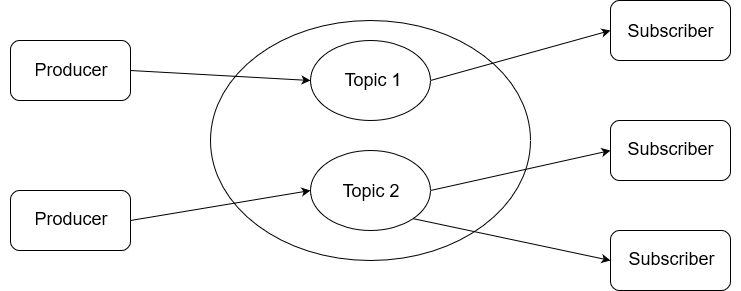
\includegraphics[scale=0.50]{img/producer_subscriber.png}
	\caption{Schéma du principe Producer/Subscriber}
	\label{Lambda}
\end{figure}

\subsubsection*{Point-to-point communication}

La communication point à point est la forme la plus simple de Producteur/Consommateur. Le producteur envoie ses données dans une queue et le consommateur va lire les messages dans la queue. Tout comme le modèle précédent, il peut y avoir plusieurs producteur et consommateurs sur la même queue, mais si plusieurs consommateurs sont présents, ils ne recevront des portions différentes des messages afin de favoriser le traitement concurrentiel.

\subsection{Kafka}

Apache Kafka~\cite{KAFKA}\cite{KAFKA2} est un système de messages distribué. Ce dernier est open source et sous licence Apache. Il a été placé sous la bannière open source par Linkedin qui continue à contribuer à son développement.

Kafka utilise le système de communication du Publisher / Subscriber.
Kafka est un cluster constitué de Brokers. Un broker est une instance d'un serveur Kafka.
Il est donc facile de se constituer un cluster Kafka en instanciant les services Kafka.
Cette gestion en cluster permet d’améliorer le partitionnement et la réplication des données.

Le partitionnement est important lorsque le volume de données va augmenter.
En utilisant un double partitionnement sur un Topic, on pourra augmenter le "débit" de lecture des messages en rajoutant un consommateur. Un consommateur s'occupera donc d'une partition d'un Topic. Cela permet aussi de facilement mettre à l'échelle Kafka si le nombre de message augmente ou si on veut accélérer le traitement.

Afin de gérer le cluster, kafka se base sur Apache Zookeeper~\cite{ZOOKEEPER} (très utilisé dans les systèmes distribués). Pour faire simple, Zookeeper permet de savoir quel service est où. Kafka , a juste à lui demandé à quel endroit est situé un certain brooker.

L'un des atout de Kafka, c'est qu'il stocke les messages.
Ce stockage est basé sur un structure de données appelé : \textbf{LOG}.
Ce format n'a rien à voir avec les logs applicatifs, il s’agit d’un tableau de messages ordonnés. L'ordonnancement est réalisé à partir de la date d'arrivée du message. Chaque message se voit donner un index, dans Kafka on appel cela un offset.

\subsection{ActiveMQ}

\subsection{RabbitMQ}

\section{Ingestion/Extraction de données}

La première catégorie, qui est aussi la première étape d'une architecture Big Data, c'est le récupération de données. Plus précisément comment nous allons récupérer des données, soit via des requêtes sur des sources externes, soit des sources externes nous envoie directement des données. 

\subsection{Apache Nifi}

\subsection{Talend}

\subsection{Solution maison}


\section{Traitement des données}

Après avoir récupérer des données, nous devons passer à l'étape du traitements des données. Celui ci à plusieurs rôles, en effet il peut servir à formater les données, leurs apportés de la cohérence en les combinant à des données déjà présentent. Et pour finir les rediriger vers le stockage souhaité. Le traitement des données peut se faire de deux manière différentes. La première solution est le traitement par Batch, et la seconde est le traitement en temps réel~\cite{TYPE_TRAITEMENT_DONNEES}. Chacune possède ses avantages et inconvénients, nous allons voir ça plus en détails.

\subsection{Batch}

Le traitement par Batch (Traitement par lot), consiste à traiter un important volume de données à un instant T. Le traitement par batch est surtout utilisé dans les cas ou nous avons des données stockés de manière journalière, et que nous avons besoin de tout traités en fin de journée. Il n'est pas rare de voir des tâches de traitements par Batch s'exécuter dans la nuit, étant donnée que l'on traite une masse de donnée importante, on sollicite la machine pendant une longue période. Réaliser ce traitement durant des périodes creuses, permet de largement diminuer l'impact sur l'utilisation de la plateforme (\ref{traitement-batch}).

\begin{figure}[!h]
	\centering 
	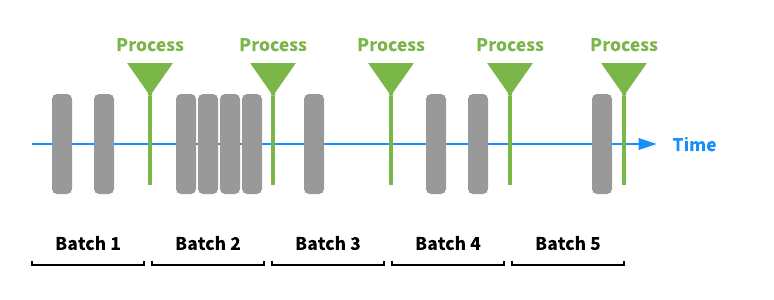
\includegraphics[scale=0.50]{img/batch-processing.png}
	\caption{Schéma du traitement par batch}
	\label{traitement-batch}
\end{figure}

Nous allons nous pencher sur les solutions existantes, implémentant un traitement par batch.

\subsubsection{Spark}

\subsubsection{Hadoop MapReduce}

\subsection{Streaming}

Un traitement de données est considéré comme étant en temps réel si il s'effectue en une seconde ou moins après la réception de la donnée. Il peut être de deux types, soit des micro batchs soit en streaming.

\subsubsection*{Micro-Batch}

Le traitement par micro batch est basé sur le même principe que le traitement par batch, à l'exception qu'il s'exécute beaucoup plus régulièrement (Toutes les secondes ou moins) et que le nombre de données à traiter est donc significativement plus faible. Le micro batch est surtout utilisé dans les cas où notre système ne peut pas directement réagir lorsqu'une donnée arrive, on va donc récupérer les données très régulièrement afin de garantir un traitement en temps réel ou du moins dans le délai le plus bref possible.

\subsubsection*{Streaming}

Le traitement en streaming (Traitement de flux), s'appuie sur l'architecture réactive ({\ref{a:architecture-reactive}}). En effet, contrairement aux traitements par batch et micro batch, ici on ne vas pas récupérer des données de temps en temps. Dès qu'une donnée arrive on va la récupérer et la traiter immédiatement. De par son fonctionnement, le traitement en streaming ne nécessite pas de stockage en amont contrairement aux autres type de traitement (\ref{traitement-streaming}).

\begin{figure}[!h]
	\centering 
	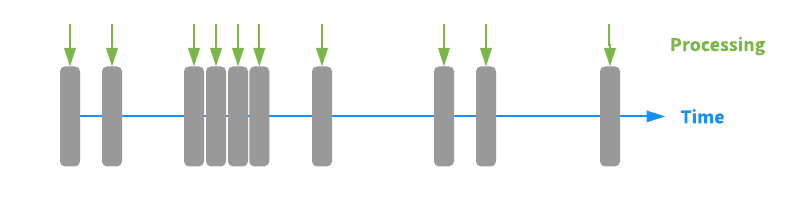
\includegraphics[scale=0.50]{img/stream-processing.png}
	\caption{Schéma du traitement en streaming}
	\label{traitement-streaming}
\end{figure}

Nous allons maintenant nous intéresser aux différentes solutions proposant ce type de traitement.

\subsubsection{Spark Streaming}

\subsubsection{Apache Storm}


\section{Stockage des données}

Une partie très importante du Big Data est le stockage des nombreuses données que l'ont reçoit. Il existe énormément de manières différentes de stocker des données selon la manière dont nous voulons les utiliser par la suite et surtout selon leurs format.

\subsection{Time Series}

\subsubsection{OpenTSDB}

\subsubsection{InfluxDB}

\subsection{Graph}

\subsubsection{Neo4j}

\subsubsection{JanusGraph}

\subsection{Clés/Valeurs}

\subsubsection{Redis}

\subsubsection{RocksDB}

\subsection{Documents}

\subsubsection{CouchDB}

\subsubsection{CouchBase}

\subsubsection{MongoDB}

\subsection{Wide Column}

\subsubsection{HBase}

\subsubsection{Cassandra}

\subsection{Système de fichiers}

\subsubsection{Hadoop HDFS}

\section{Orchestration}

\section{Requetâge}

\section{Visualisation et Analyse des données}

\subsection{Kibana}

\subsection{Banana}

\subsection{Grafana}

\subsection{Tableau}

\subsection{Click}